% Print results for GEB estimates for F-norm^2

\begin{figure}[p]
    \centering

    \begin{subfigure}{0.45\textwidth}
    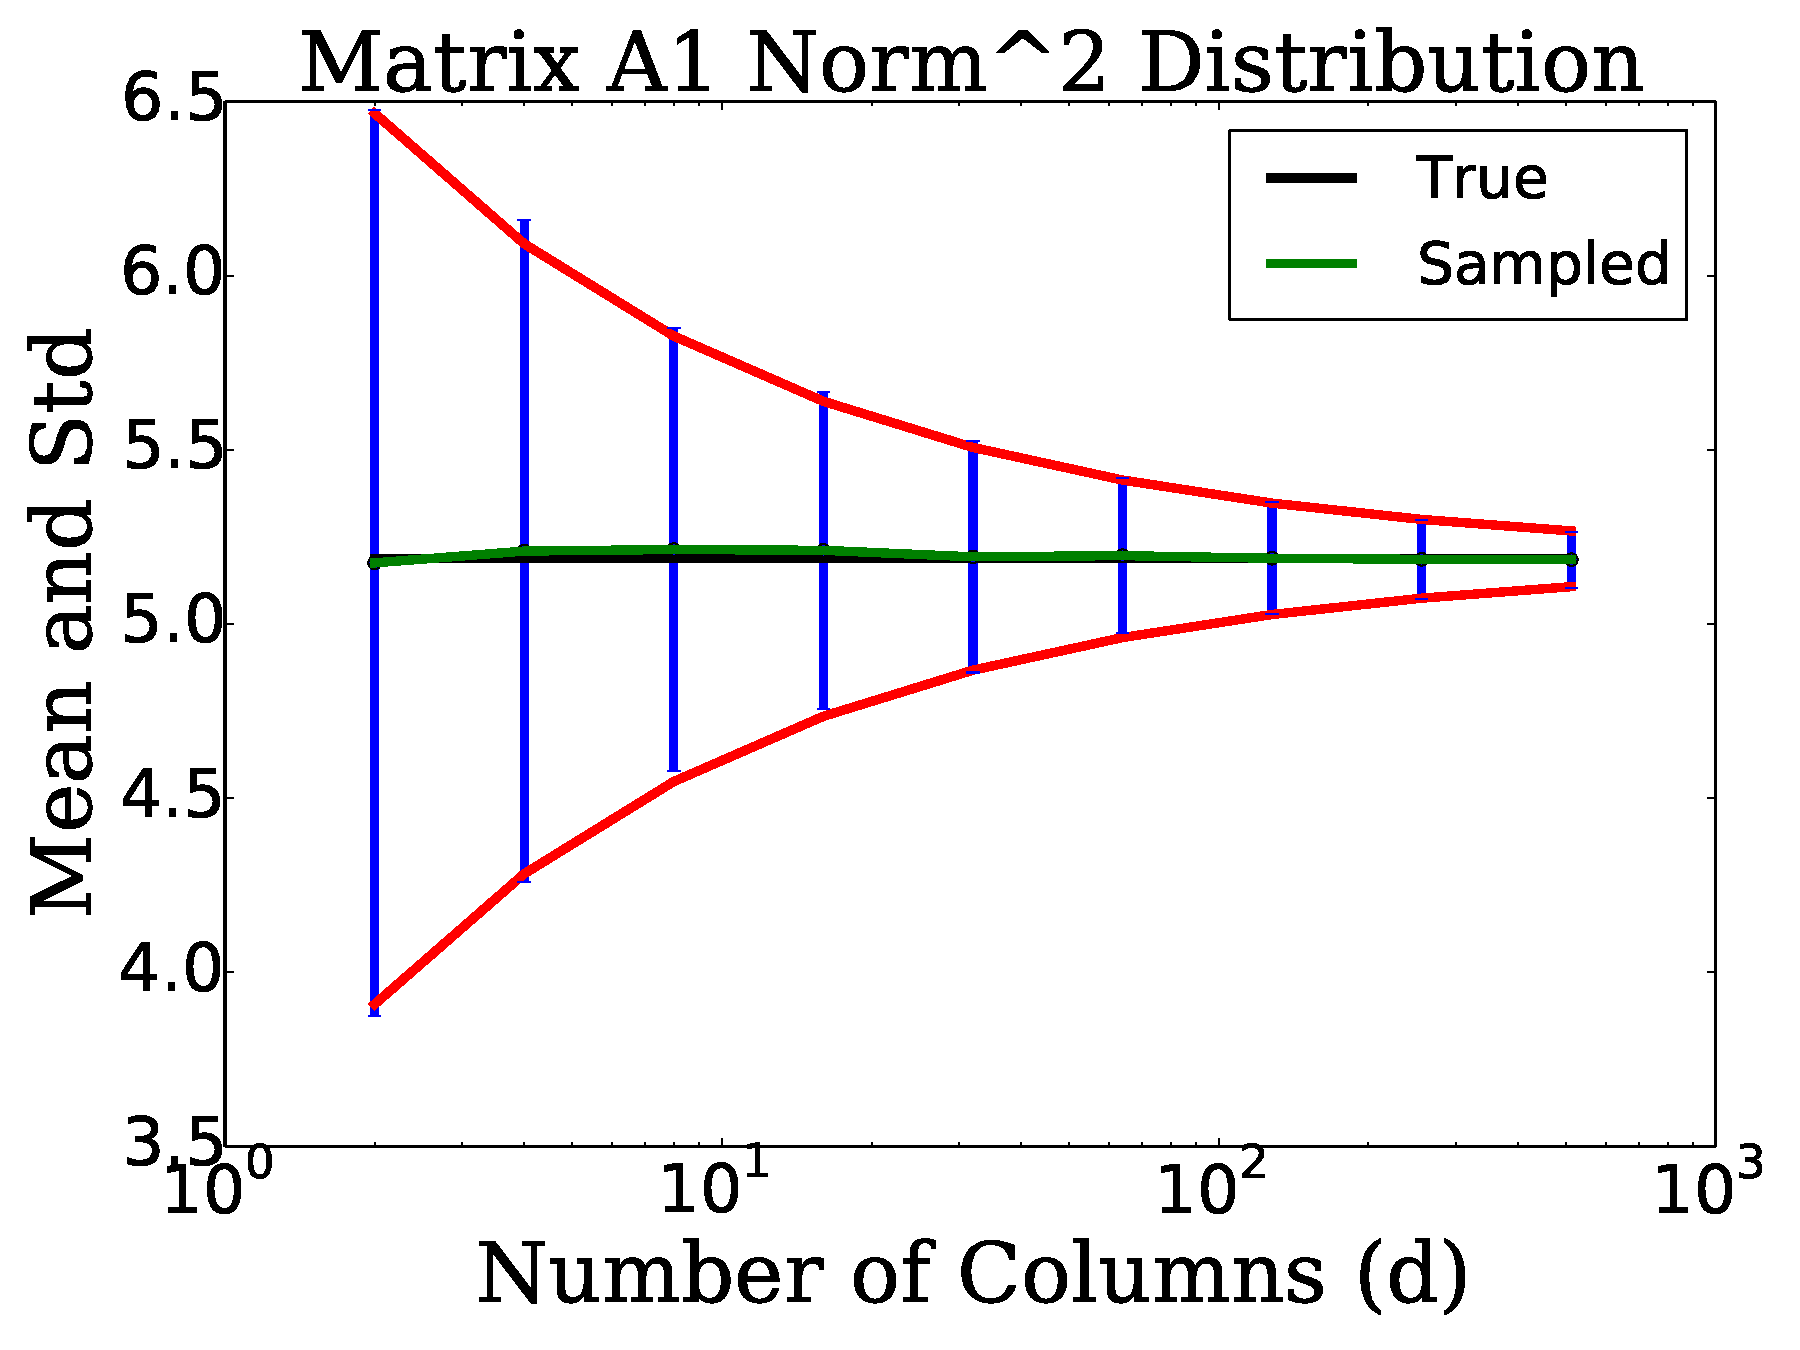
\includegraphics[width=\textwidth]{plots/mat_A1_error_test_2.pdf}
    \caption{Matrix A1}
    \end{subfigure}
    \begin{subfigure}{0.45\textwidth}
    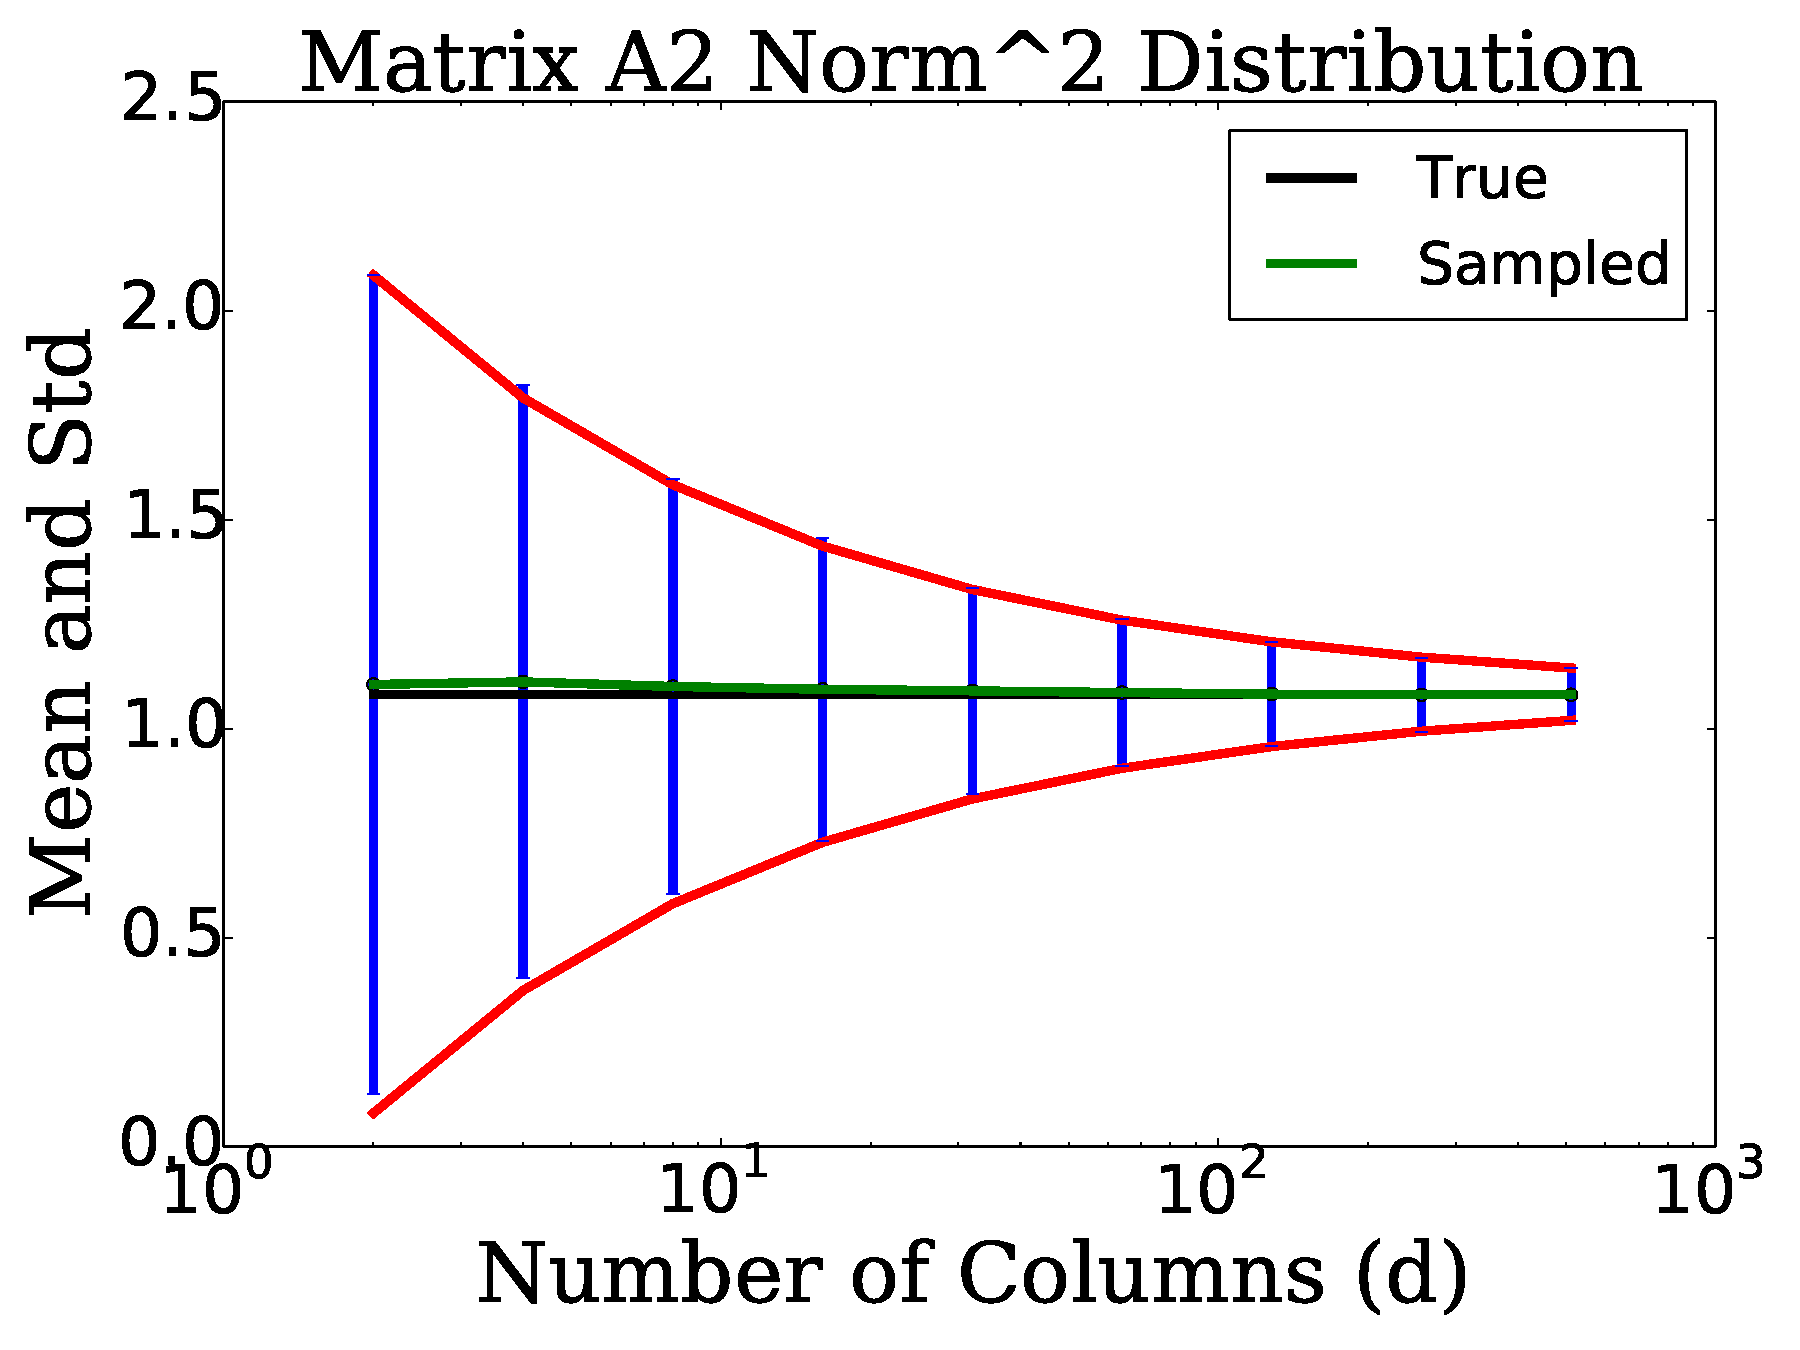
\includegraphics[width=\textwidth]{plots/mat_A2_error_test_2.pdf}
    \caption{Matrix A2}
    \end{subfigure}

    \begin{subfigure}{0.45\textwidth}
    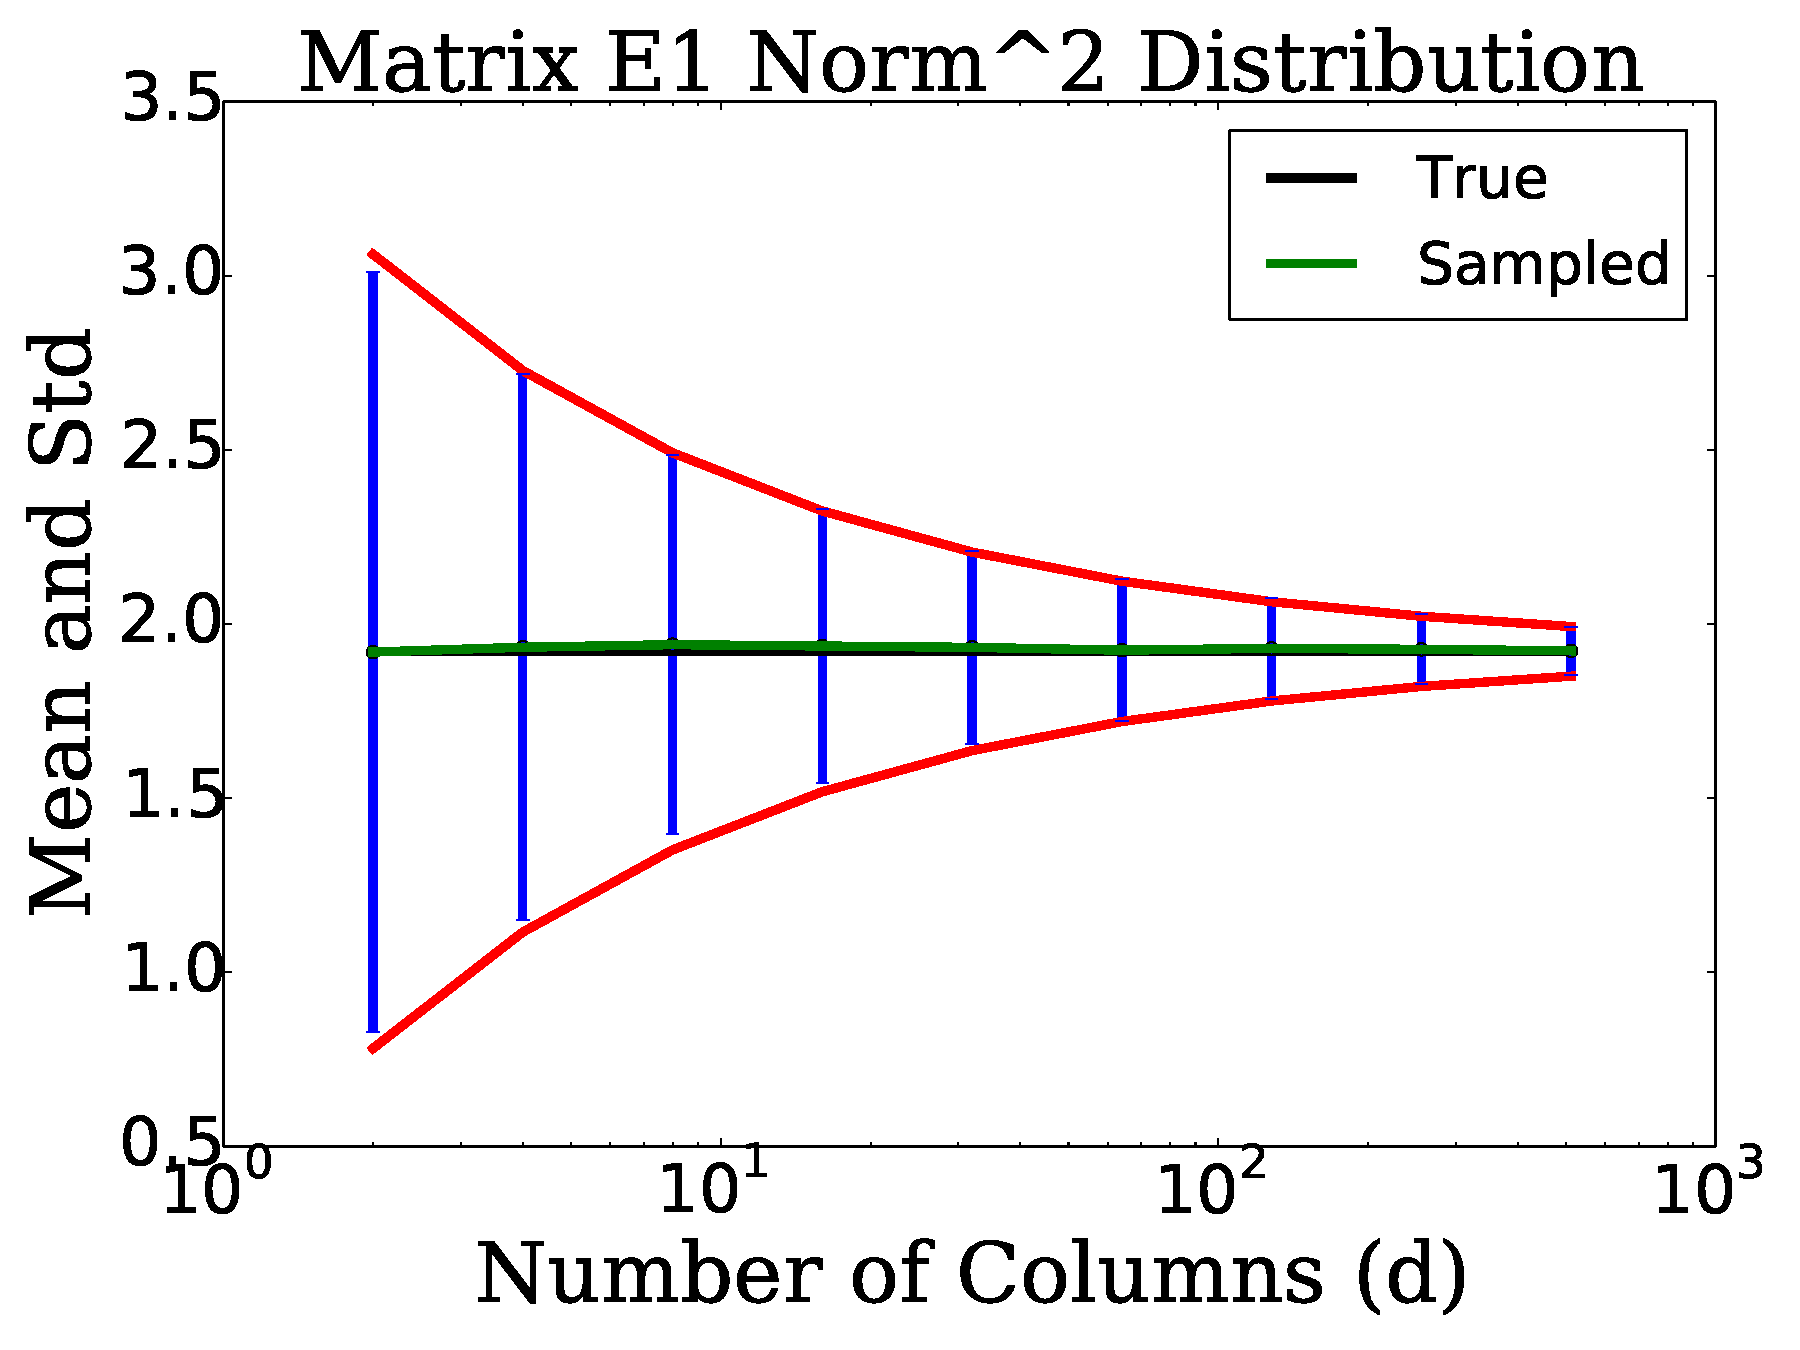
\includegraphics[width=\textwidth]{plots/mat_E1_error_test_2.pdf}
    \caption{Matrix E1}
    \end{subfigure}
    \begin{subfigure}{0.45\textwidth}
    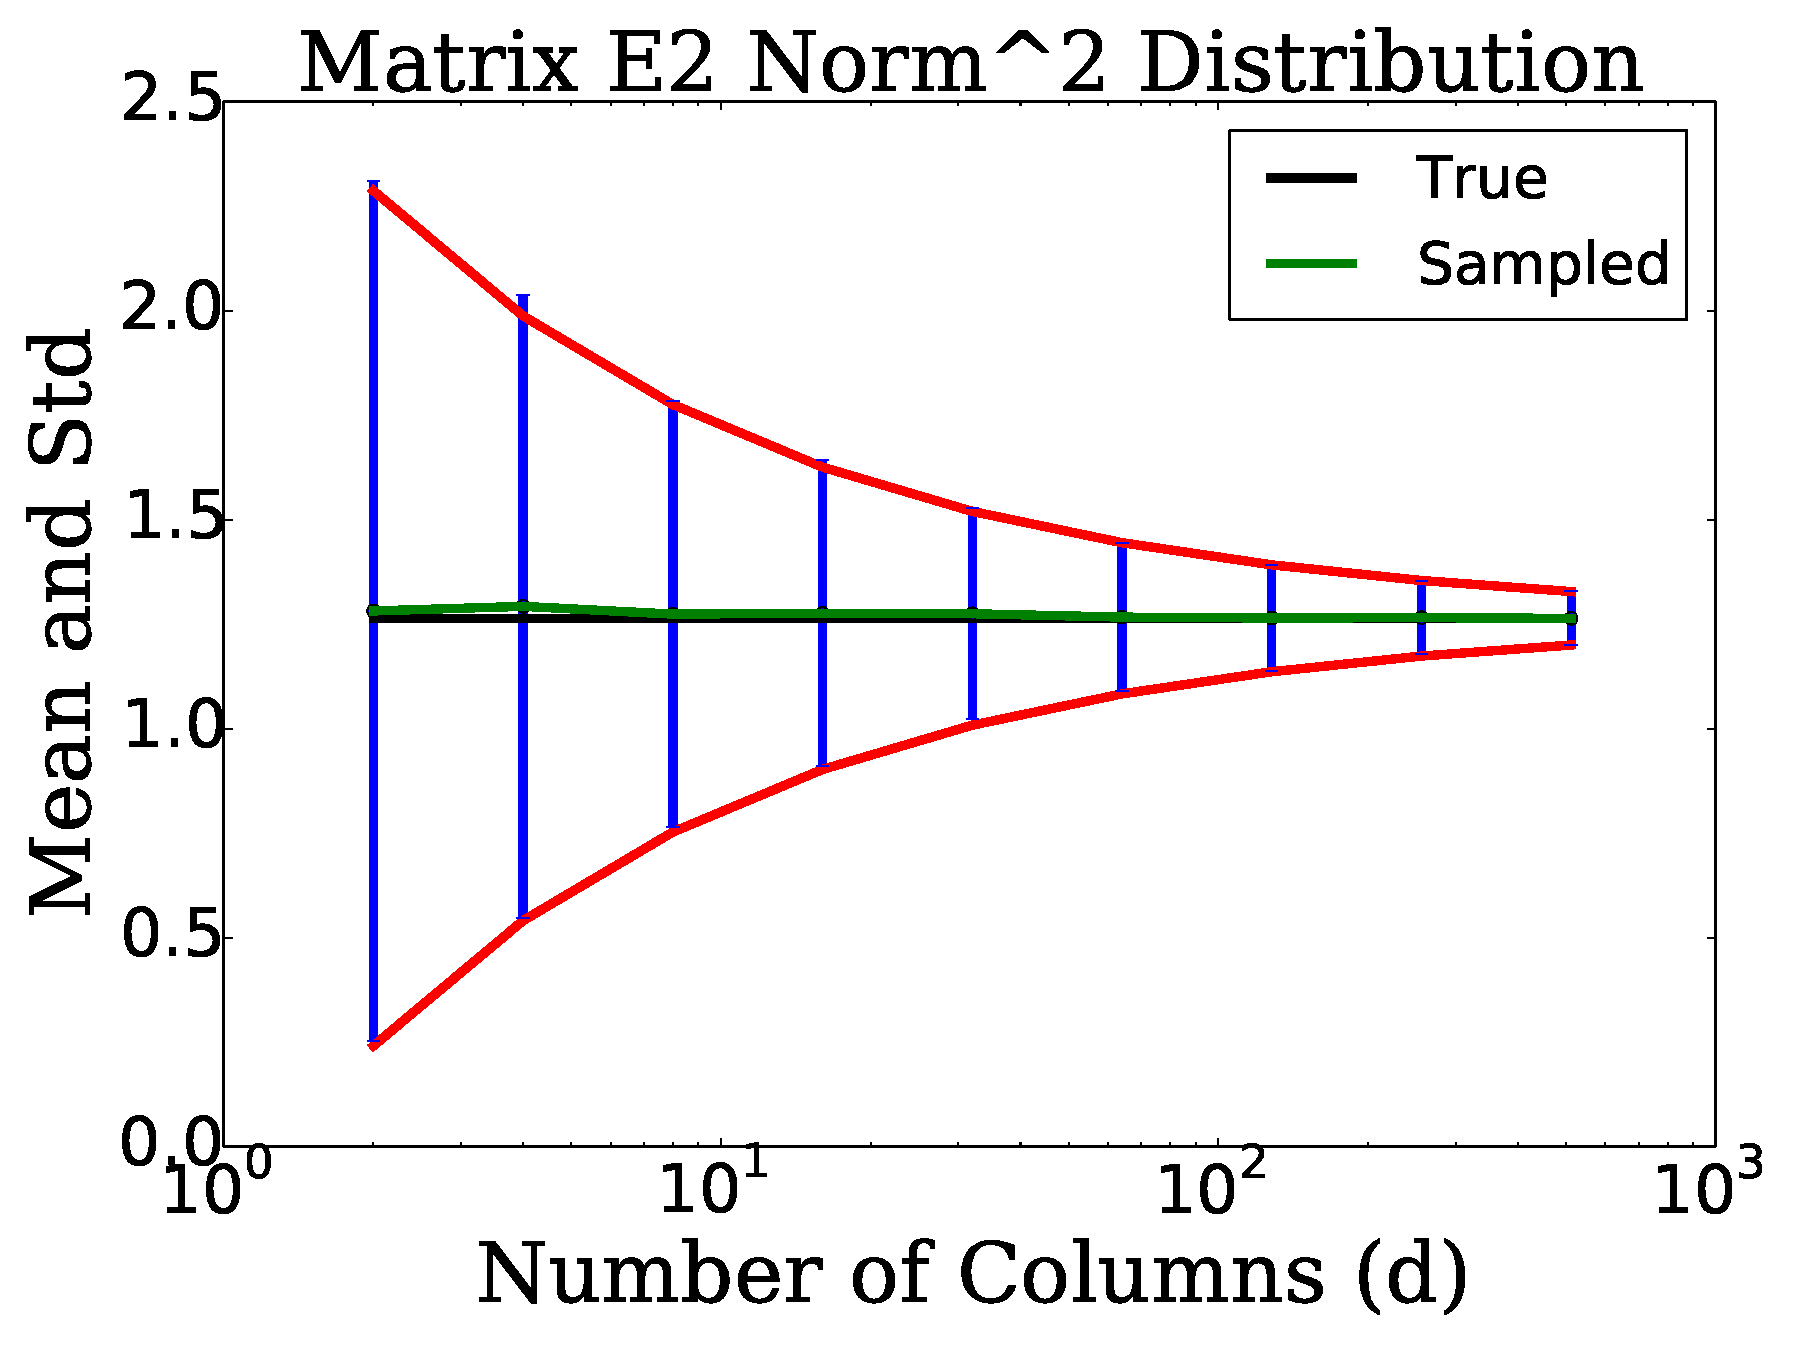
\includegraphics[width=\textwidth]{plots/mat_E2_error_test_2.pdf}
    \caption{Matrix E2}
    \end{subfigure}

    \begin{subfigure}{0.45\textwidth}
    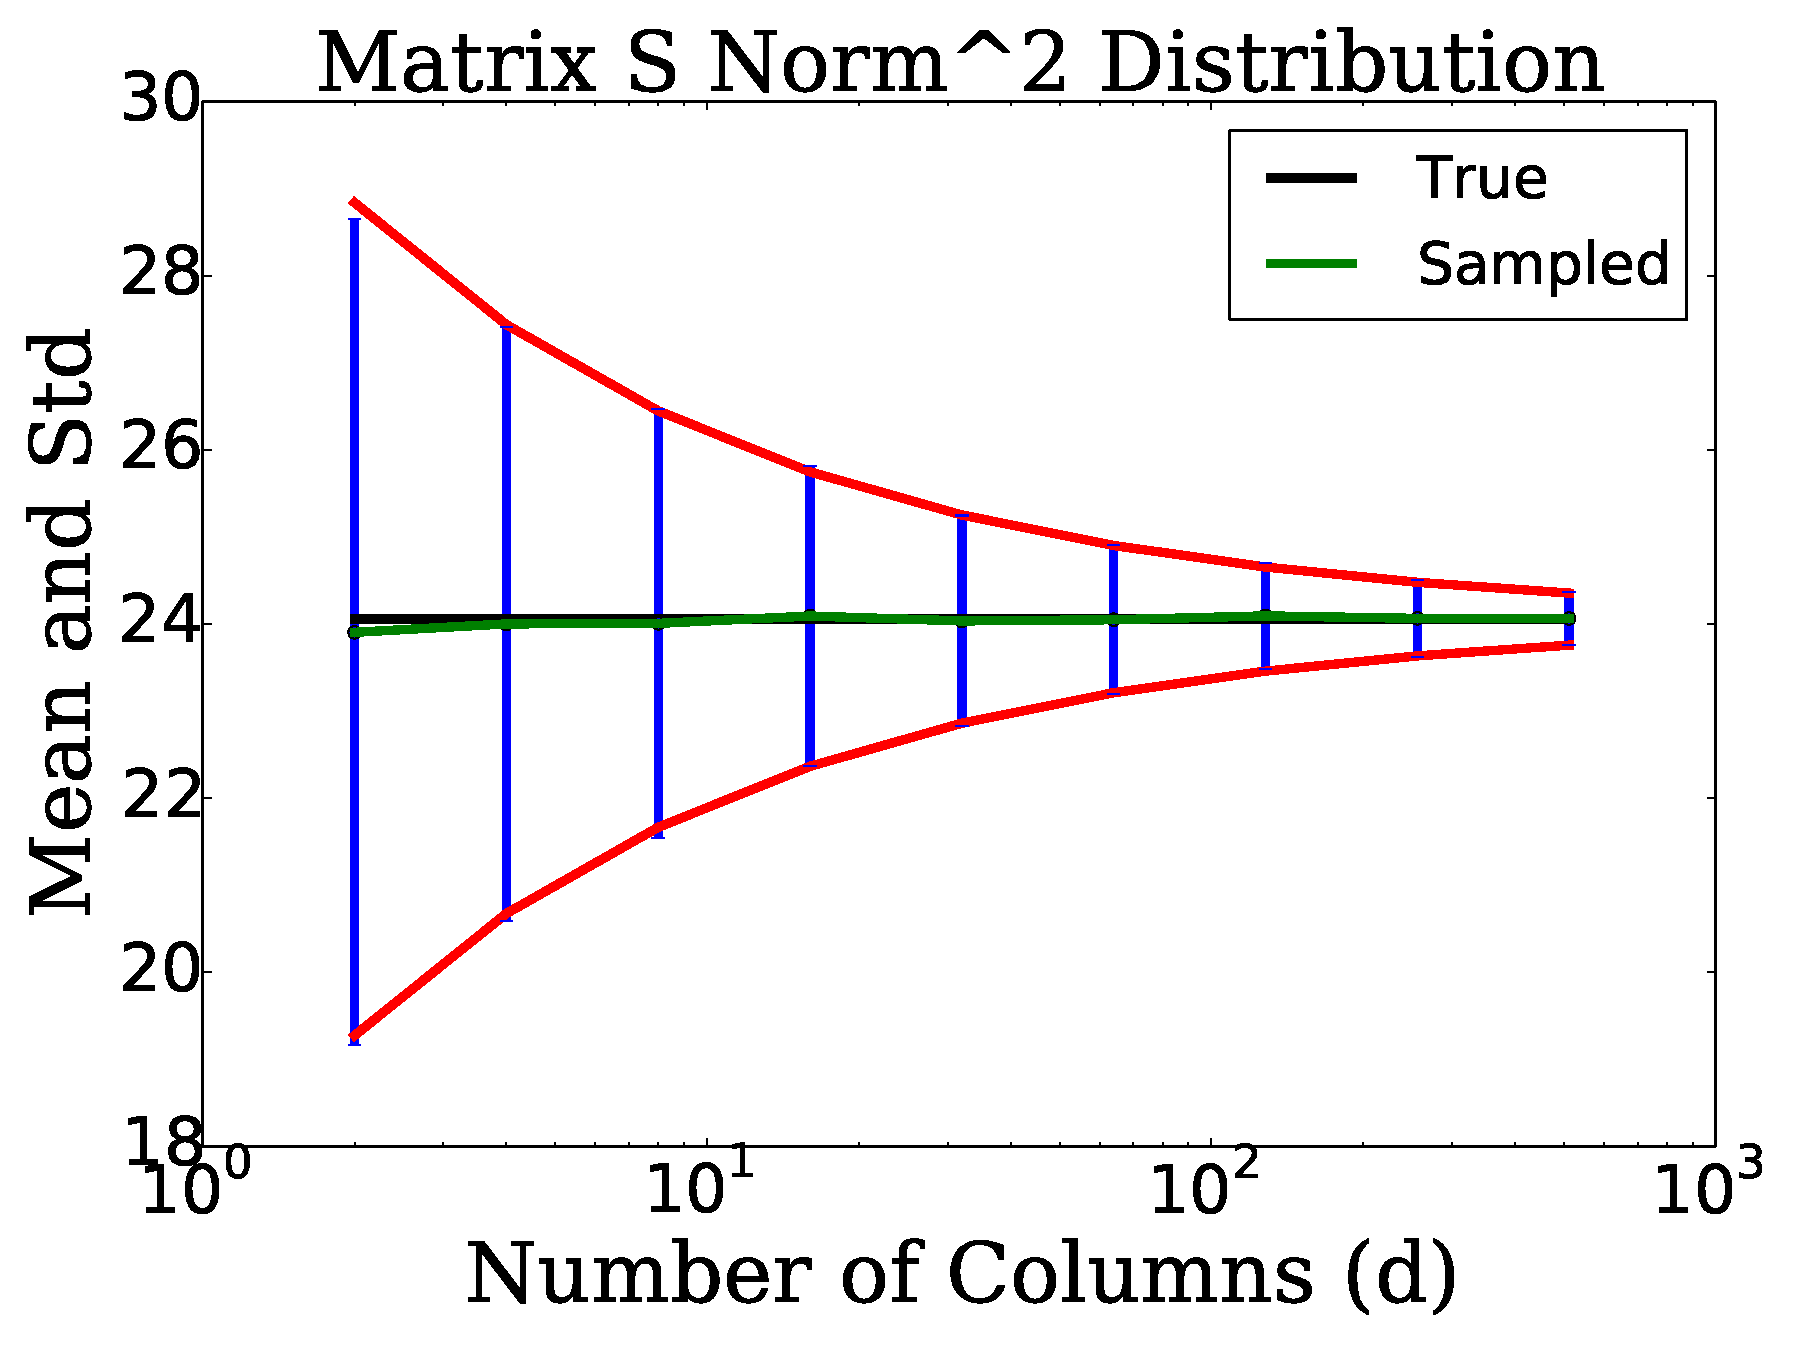
\includegraphics[width=\textwidth]{plots/mat_S_error_test_2.pdf}
    \caption{Matrix S}
    \end{subfigure}
    \begin{subfigure}{0.45\textwidth}
    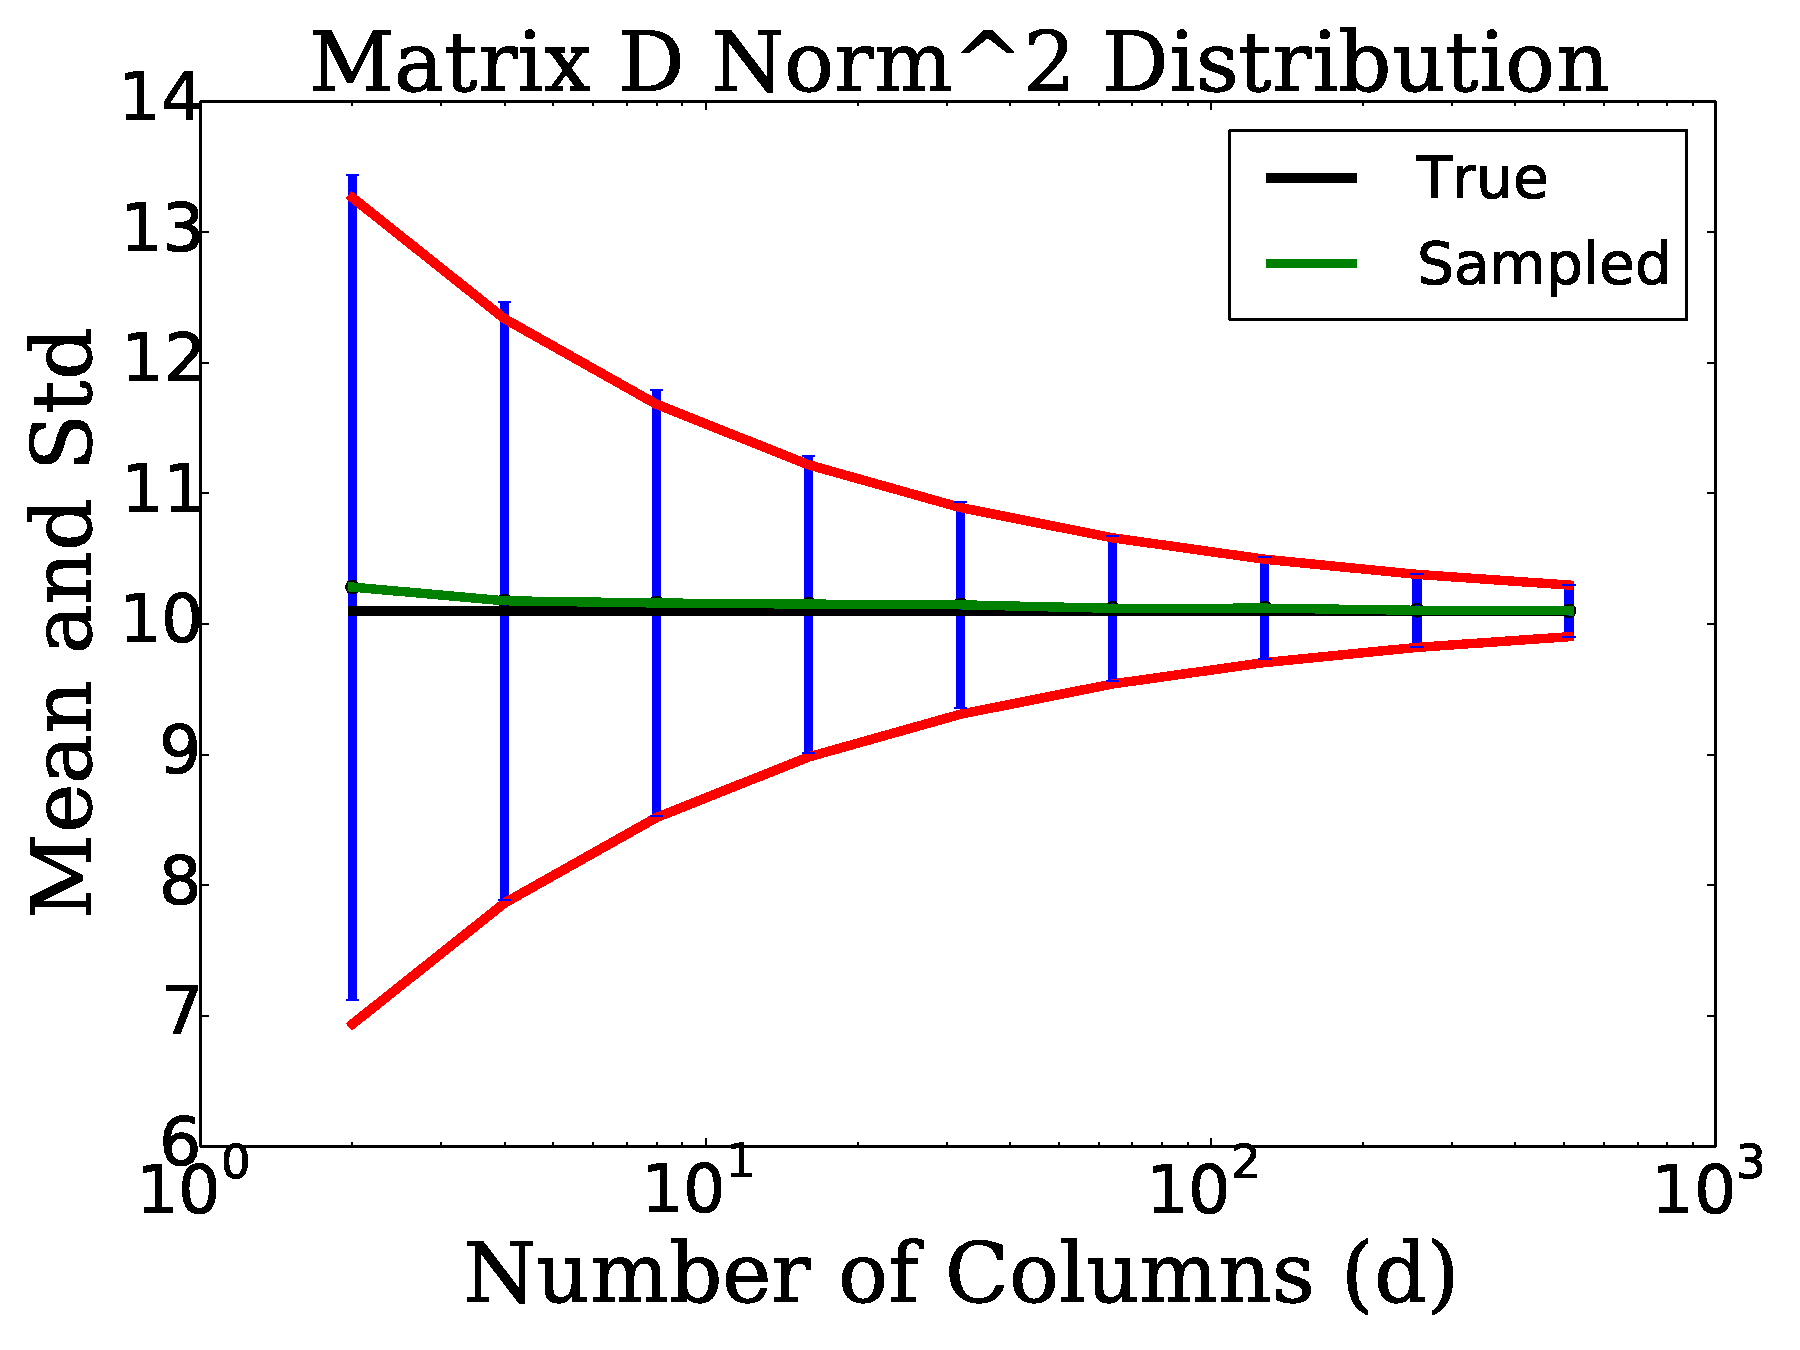
\includegraphics[width=\textwidth]{plots/mat_D_error_test_2.pdf}
    \caption{Matrix D}
    \end{subfigure}

\caption[GEB Stochastic Squared F-norm Approximations]{
%Estimated $||A||_{F}$ for our matrices using the Gaussian Error Bound.
We performed 10,000 trials and computed the
mean (Green) and standard deviation (Blue) of $\norm{A\Omega}_{F}^{2}$
for columns $d\in\{2,4,8,\cdots,512\}$.
The true squared F-norm value is Black and the theoretical standard
deviation bounds from Eq.~\eqref{eq:rand_Xd_variance_bounds} are Red.
}
\label{fig:geb_norm_squared_bound_mat}
\end{figure}



